%\documentclass[10pt]{article}
\documentclass[fleqn]{article}
%\usepackage[cm]{fullpage}
\usepackage{graphicx}
\usepackage{amsmath}
\usepackage{outlines}
\usepackage{listings}
%\usepackage{xcolor}
\usepackage[table]{xcolor}

\usepackage{multirow}
\usepackage{multicol}
\usepackage{booktabs}
\lstset { %
	language=R,
	backgroundcolor=\color{black!5}, % set backgroundcolor
	basicstyle=\footnotesize,% basic font setting
}

%Regression table preamp
\usepackage{pdflscape}
\usepackage{booktabs} % For \toprule, \midrule and \bottomrule
\usepackage{siunitx} % Formats the units and values
\usepackage{pgfplotstable} % Generates table from .csv
\usepackage{booktabs}

%\documentclass[preprint,floatfix] {revtex4} 
\newcommand{\rvec}{\mathrm {\mathbf {r}}} 
\usepackage{subfigure}
\usepackage{color, soul}


% Setup siunitx:
\sisetup{
	round-mode          = places, % Rounds numbers
	round-precision     = 4, % to 2 places
}

\usepackage{float}

\title{Housing and Credit Cycles}
\author{Nam Nguyen}
\date{\today}                                          

\begin{document}
	\maketitle
	
	\begin{outline}[enumerate]
		
		\section{Motivation}
		
		This paper uses a multivariate extension of the model proposed by Morley et al. (2003) and Huang and Kishor (2018)
		
		The novel contribution of this paper is the inclusion of cross transitory components effect as seen in eq(5) \& eq(6). I would like to take advantage of it to explore the dynamics of the relationship between housing prices and house hold credit in the short run.
		
		\section {Model Specification}
		
		\textbf{\textit{Series:}} \\
		-Credit : Credit to non financial sector\\
		-HPI : Housing Price Index
		\begin{align}
		ln \frac{Credit}{GDP} &= y_t = \tau_{yt} + c_{yt}
		\\
		ln HPI &= h_t = \tau_{ht} + c_{ht}
		\end{align}
		\\
		\textbf{\textit{Trends:}}
		
		A random walk drift term $g_t$ is added in the stochastic trend inspired by Clark (1987)
		\begin{align}
		\tau_{yt} &= \tau_{yt-1} + \eta_{yt}, &\eta_{yt} \sim iidN(0,\sigma^2_{\eta y})
		\\
		\tau_{ht} &= \tau_{ht-1} + \eta_{ht}, &\eta_{ht} \sim iidN(0,\sigma^2_{\eta h})	
		\end{align}
		\\
		\textbf{\textit{Cycles:}}
		\begin{align}
		c_{yt} &= \phi^1_{y}c_{yt-1}  
		+ \phi^2_{y}c_{yt-2}  
		+ \phi^x_{y}c_{ht-1} 
		+ \varepsilon_{yt},
		&\varepsilon_{yt} \sim iidN(0,\sigma^2_{\varepsilon y})		   
		\\
		c_{ht} &= \phi^1_{h}c_{ht-1}  
		+ \phi^2_{h}c_{ht-2}
		+ \phi^x_{h}c_{yt-1}  
		+ \varepsilon_{ht},
		&\varepsilon_{ht} \sim iidN(0,\sigma^2_{\varepsilon h})
		\end{align}
		\\
		
		
		\textbf{State-Space Model}
		
		\textit{Transition equation:}
		\begin{align}
		\beta_t = F\beta_{t-1} + \tilde{v}_t
		\end{align}
		
		Where the transitory components are:
		
		\begin{align}
		\begin{bmatrix}
		\tau_{yt}	\\
		c_{yt}		\\
		c_{yt-1}		\\
		\tau_{ht}	\\
		c_{ht}		\\
		c_{ht-1}		
		\end{bmatrix}
		=
		%F matrix
		\begin{bmatrix}
		1	& 0	& 0	& 0	& 0	& 0	\\
		0	& \phi^1_y	& \phi^2_y	& 0	& \phi^x_y	& 0	\\
		0	& 1	& 0	& 0 & 0 & 0  \\
		0	& 0	& 0	& 1	& 0	& 0 \\
		0	& \phi^x_h	& 0	& 0 &\phi^1_h	& \phi^2_h	\\
		0	& 0	& 0	& 0 & 1 & 0
		\end{bmatrix}
		%Bt-1 matrix
		\begin{bmatrix}
		\tau_{yt-1}	\\
		c_{yt-1}		\\
		c_{yt-2}		\\
		\tau_{ht-1}	\\
		c_{ht-1}		\\
		c_{ht-2}		
		\end{bmatrix}
		+
		\begin{bmatrix}
		\eta_{yt}	\\
		\varepsilon_{yt}		\\
		0	\\
		\eta_{ht}	\\
		\varepsilon_{ht}		\\
		0	
		\end{bmatrix}
		\end{align}
		
		\textit{The covariance matrix for $\tilde{v}_t$, denoted Q, is: }
		\begin{align}
		Q = 
		\begin{bmatrix}
		\sigma^2_{\eta y}	& 0	 &0 & 0	& 0	& 0	\\
		0	& \sigma^2_{\varepsilon y}	& 0	& 0	& \sigma_{\varepsilon y \varepsilon h}	& 0	\\
		0	&	0	& 0 & 0 & 0 & 0	\\
		0	& 0	& 0	& \sigma^2_{\eta h}	& 0	& 0	\\
		0	& \sigma_{\varepsilon y \varepsilon h}	& 0	& 0	& \sigma^2_{\varepsilon h}		& 0	\\
		0	&0	& 0	& 0
		& 0	& 0
		\end{bmatrix}
		\end{align}
		
		\textit{Measurement Equation:}
		\begin{align}
		\tilde{y}_t = A + H\beta_t
		\end{align}
		
		\begin{align*}
		\begin{bmatrix}
		y_t	\\
		h_t
		\end{bmatrix}
		=
		\begin{bmatrix}
		0	\\
		0
		\end{bmatrix}
		+
		\begin{bmatrix}
		1	& 0	& 1	& 0	& 0 & 0 \\
		0	& 0 & 0 & 1 & 0 & 1
		\end{bmatrix}
		\begin{bmatrix}
		\tau_{yt}	\\
		c_{yt}		\\
		c_{yt-1}	\\
		\tau_{ht}	\\
		c_{ht}		\\
		c_{ht-1}
		\end{bmatrix}
		\end{align*}
		\pagebreak
\section{Parameters constraints}

The estimation of the unobserved component model uses a nonlinear log-likelihood function maximization. Estimating this function requires numerical optimization.


I did not put stationary constraints directly on the autoregressive parameters. Since such constraints on a VAR(2) system is complex to setup. However, to achieve feasible stationary transitory measurement, I implement an additional term on the objective function:

\begin{align}
l(\theta) = -\frac{1}{2}\sum_{t=1}^{T}ln\lbrack(2\pi)^2|f_{t|t-1}|\rbrack
-\frac{1}{2}\sum_{t=1}^{T}\eta'_{t|t-1}f^{-1}_{t|t-1}\eta_{t|t-1}
- 0.003*\sum_{t=1}^{T}(c_{yt}^2+c_{ht}^2)
\end{align}

The last term in the objective function acts as a penalty against too much transitory deviation from zero. Without this penalty, the trend would be linear or all the movements in the measured series would be matched by transitory movements.

\vspace{5mm} %5mm vertical space

Regarding constraints on covariance matrix, I applied the same constraints as in Morley 2007 to imply for positive definite matrix.


\section{Priors selection}

The priors for autoregressive parameters in matrix F are taken from VAR regression of the HP filter cycle decomposition of the series.

For $\beta_{0|0}$, I set $\tau_{0|0}$ as the value of the first available row of data and omit the first observation from the regression. $c_{0|0}$ are set to be equal to their HP filter counterpart. $var(\tau_{0|0}) =100+50*random$; while other measures of the starting covariance are set to be their unconditional values.

Starting standard deviation and correlation values are randomized within reasonable range.

		
		
		\section{Regression results}
		
		In this following section, I will apply the UC model to data from 6 countries: US, UK, Germany, France, Japan and South Korea.
		
		The estimated parameters vary greatly as I uniformly randomized priors for the MLE process. The following estimates are selected in the manner that they would look the most stable. Perhaps a more optimal constraint on the autoregressive parameters would solve this issue.
		
		The regression table below shows Unobserved component VAR(2) regression results with and without cross-cycle parameters.
		
		\pagebreak
		
		
		\begin{landscape}
			
			%Regression table
			% Please add the following required packages to your document preamble:
			% \usepackage{booktabs}
			% \usepackage{multirow}
			\begin{table}[]
				\caption {\label{tab:table1} United States regression results} 
				\rowcolors{2}{gray!10}{white}
				\begin{tabular}{@{}lSSSSSS@{}}
					\toprule
					\multirow{2}{*}{Parameters} & \multicolumn{2}{c}{VAR(2)} & \multicolumn{2}{c}{VAR(2) 1st-cross-lag} & \multicolumn{2}{c}{VAR(2) 2-cross-lags} \\
					& \multicolumn{1}{l}{Estimate}     & \multicolumn{1}{l}{Std. Error}  & \multicolumn{1}{l}{Estimate}            & \multicolumn{1}{l}{Std. Error}         & \multicolumn{1}{c}{Estimate}            & \multicolumn{1}{c}{Std. Error}        \\ \midrule
					$\phi^1_{y}$                & 1.521670374  & 0.323602024 & 1.890301193         & 0.036315042        & 1.886592178         & 0.00028419        \\
					$\phi^2_{y}$                & -0.592177551 & 0.282758652 & -0.773199508        & 0.021652307        & -0.8941981          & 0.003233388       \\
					$\phi^{x1}_{y}$             &              &             & -0.012689515        & 0.001245419        & 0.04280046          & 0.000520376       \\
					$\phi^{x2}_{y}$             &              &             &                     &                    & -0.040322766        & 0.000876719       \\
					$\phi^1_{h}$                & 1.803961772  & 0.039406338 & 1.465513594         & 0.064627659        & 1.864726867         & 0.038659834       \\
					$\phi^2_{h}$                & -0.820986013 & 0.039263457 & -0.736886204        & 0.047825955        & -0.898033258        & 0.039051475       \\
					$\phi^{x1}_{h}$             &              &             & 2.576890191         & 1.642027848        & 0.089729346         & 0.11453162        \\
					$\phi^{x2}_{h}$             &              &             &                     &                    & -0.031982418        & 0.113620129       \\
					$\sigma_{ny}$               & 0.968115538  & 0.064573932 & 0.975833563         & 0.066722551        & 0.858997834         & 0.055437867       \\
					$\sigma_{ey}$               & 0.136584746  & 0.073940054 & 0.000413197         & 0.008728546        & 0.030583756         & 0.016664357       \\
					$\sigma_{nh}$               & 0.964325946  & 0.107167236 & 1.271977495         & 0.127987617        & 1.135553581         & 0.106041662       \\
					$\sigma_{eh}$               & 0.471089742  & 0.079046967 & 0.296047479         & 0.161613716        & 0.363776038         & 0.077466523       \\
					$\sigma_{eyeh}$             & -0.999391959 & 0.03023235  & -0.881232755        & 0.311836698        & -1                  & 5.19E-07          \\
					$\sigma_{nynh}$             & 0.464225409  & 0.094391207 &                     &                    &                     &                   \\
					Log-likelihood value        & -369.9163016 &             & -384.7973521        &                    & -363.3991125        &                   \\ \bottomrule
				\end{tabular}
			\end{table}
			
		\end{landscape}
		
		\pagebreak
		
		
		\pagebreak
		
		\begin{landscape}
			
			%Regression table
			\begin{table}[]
				\caption {\label{tab:table1} Great Britain regression results} 
				\begin{tabular}{@{}lSSSSSS@{}}
					\toprule
					\multirow{2}{*}{Parameters} & \multicolumn{2}{c}{VAR(2)} & \multicolumn{2}{c}{VAR(2) 1st-cross-lag} & \multicolumn{2}{c}{VAR(2) 2-cross-lags} \\
					& \multicolumn{1}{l}{Estimate}     & \multicolumn{1}{l}{Std. Error}  & \multicolumn{1}{l}{Estimate}            & \multicolumn{1}{l}{Std. Error}         & \multicolumn{1}{c}{Estimate}            & \multicolumn{1}{l}{Std. Error}        \\ \midrule
					$\phi^1_{y}$         & 1.254192973  & 0.190985842 & 1.25723532   & 0.060817683 & 1.150590314  & 0.176355128 \\
					$\phi^2_{y}$         & -0.26306956  & 0.205161023 & -0.169780952 & 0.09490575  & -0.29219579  & 0.186002808 \\
					$\phi^{x1}_{y}$      &              &             & -0.032263112 & 0.011998484 & -9.25E-05    & 0.040559508 \\
					$\phi^{x2}_{y}$      &              &             &              &             & 0.001258809  & 0.049929897 \\
					$\phi^1_{h}$         & 1.624898849  & 0.106882442 & 0.680349073  & 0.111110636 & 0.37903173   & 0.134445053 \\
					$\phi^2_{h}$         & -0.735672409 & 0.11638218  & -0.058077279 & 0.119413569 & -0.513222468 & 0.172990361 \\
					$\phi^{x1}_{h}$      &              &             & 1.095293496  & 0.644515947 & 1.042175029  & 0.959665092 \\
					$\phi^{x2}_{h}$      &              &             &              &             & -0.24951917  & 1.444350906 \\
					$\sigma_{ny}$        & 0.860787938  & 0.082136594 & 1.144314466  & 0.116163949 & 0.739935351  & 0.04023517  \\
					$\sigma_{ey}$        & 0.289375924  & 0.120450619 & 0.192749525  & 0.076274126 & 0.475181328  & 0.106178287 \\
					$\sigma_{nh}$        & 2.340082466  & 0.172292974 & 2.162565122  & 0.187483055 & 1.423757795  & 0.059105068 \\
					$\sigma_{eh}$        & 0.75058414   & 0.220465076 & 1.898423971  & 0.342466946 & 2.079589016  & 0.470123296 \\
					$\sigma_{eyeh}$      & 0.957116136  & 0.252780005 & 0.502139385  & 0.163311142 & 0.48533368   & 0.153929437 \\
					$\sigma_{nynh}$      & 0.591929269  & 0.07200974  &              &             &              &             \\
					Log-likelihood value & -410.01474   &             & -448.3113461 &             & -512.4696846 &                             \\ \bottomrule
				\end{tabular}

			\end{table}
			
		\end{landscape}
		
		\clearpage
		
		Given the regression results from the above table. To avoid the problem of perfect collinearity as shown in US data regression, and also to have a more significant estimate of the cross cycle component; I select the second model - VAR(2) with 1 cross lag in the cycle component as the one to focus on.
		
		The novel contribution of this paper is to introduce this parameter $\phi^{x1}_h$ in which it measure the effect of a change in last period credit transitory component on the current housing price transitory component. In both regressions in the US and GB, I can observe that there is a nearly significant positive effect of last period credit cycle deviation on current housing cycle component.
		\\
		
		The following graphs shows the UC forecast series against the actual data series.
		
		\begin{figure}[h!]
			\caption{VAR(2) cross-cycle 1st lag US: Cycle components}	
			\centerline{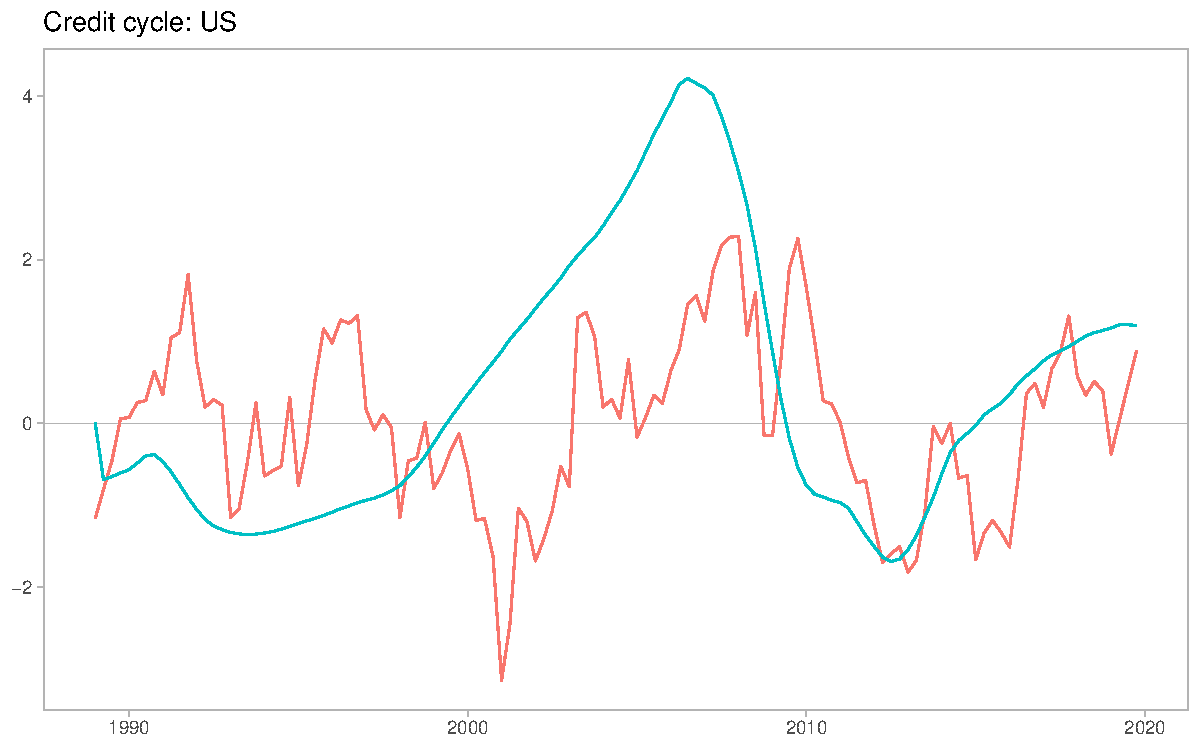
\includegraphics[scale=0.7]{../../Regression/VAR_2_crosscycle_1stlagonly/Output/Graphs/Credit_cycle_US.pdf}}
			\centerline{\includegraphics[scale=0.7]{../../Regression/VAR_2_crosscycle_1stlagonly/Output/Graphs/HP_Cycle_US.pdf}}
		\end{figure}
		
		\begin{figure}[h!]
			\caption{VAR(2) cross-cycle 1st lag US: Trend components}	
			\centerline{\includegraphics[scale=0.7]{../../Regression/VAR_2_crosscycle_1stlagonly/Output/Graphs/Credit_trend_US.pdf}}
			\centerline{\includegraphics[scale=0.7]{../../Regression/VAR_2_crosscycle_1stlagonly/Output/Graphs/HP_trend_US.pdf}}
		\end{figure}
		
		\begin{figure}[h!]
			\caption{VAR(2) cross-cycle 1st lag GB: Cycle components}	
			\centerline{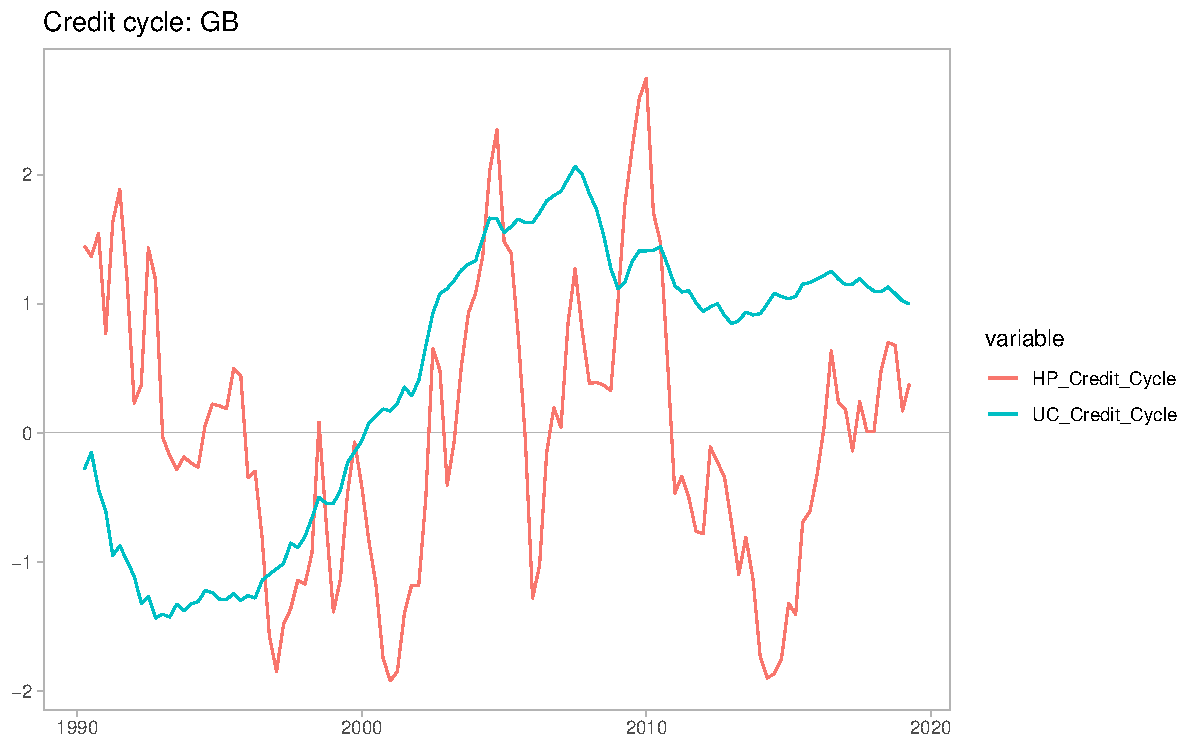
\includegraphics[scale=0.7]{../../Regression/VAR_2_crosscycle_1stlagonly/Output/Graphs/Credit_cycle_GB.pdf}}
			\centerline{\includegraphics[scale=0.7]{../../Regression/VAR_2_crosscycle_1stlagonly/Output/Graphs/HP_Cycle_GB.pdf}}
		\end{figure}
		
		\begin{figure}[h!]
			\caption{VAR(2) cross-cycle 1st lag GB: Trend components}	
			\centerline{\includegraphics[scale=0.7]{../../Regression/VAR_2_crosscycle_1stlagonly/Output/Graphs/Credit_trend_GB.pdf}}
			\centerline{\includegraphics[scale=0.7]{../../Regression/VAR_2_crosscycle_1stlagonly/Output/Graphs/HP_trend_GB.pdf}}
		\end{figure}
		
		\clearpage
		\section{Conclusion}
		Employing cross effects on the transitory components of the two series allows me to measure the effect of short term shock from house hold credit on housing price and vice versa.
				
		In this paper, the models for US and GB data shows that there is a positive relationship between a one period lag in short term house hold credit and house price. 
		
		Further development for this paper should include more robust optimal constraints on parameters to ensure stability. 
		
		Additionally, comparison in term of fitness and prediction error with other model such as a conventional multivariate UC model, univariate UC model, AR(2) model could be done in order gauge the benefit of including extra variables in the transitory component.
		
				
		\section*{Appendix}

		I will also include graphs that compare the 3 regression models forecast against HP filter cycle components.
		
		\clearpage
		
		
		\begin{figure}[h!]
			\caption{VAR(2) cross-cycle US: Cycle components}	
			\centerline{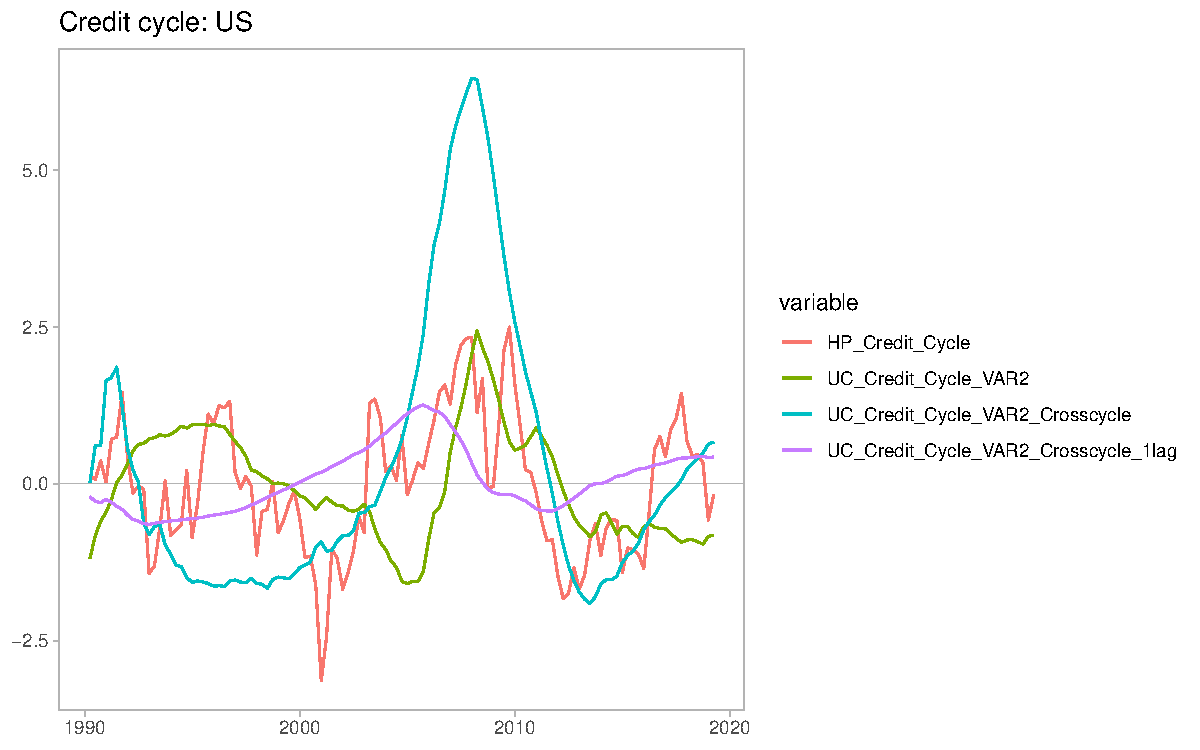
\includegraphics[scale=0.7]{../Graphs/Credit_cycle_US.pdf}}
			\centerline{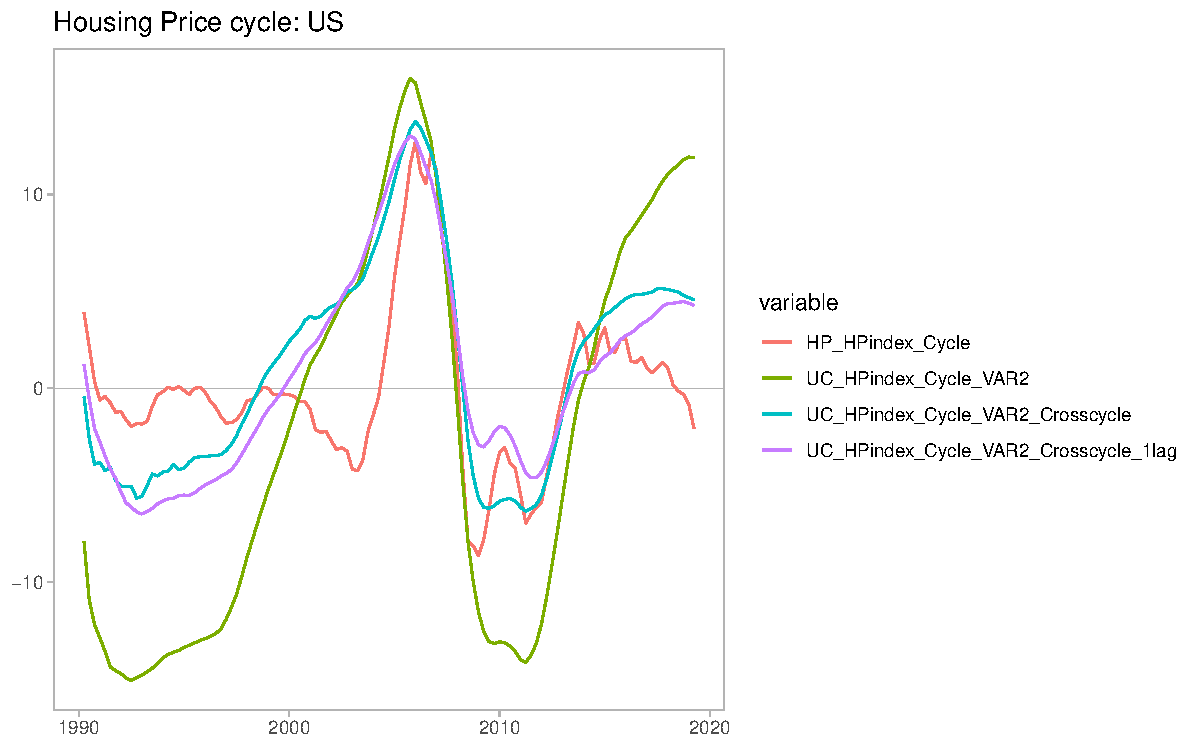
\includegraphics[scale=0.7]{../Graphs/HP_cycle_US.pdf}}
		\end{figure}
		
		\begin{figure}[h!]
			\caption{VAR(2) cross-cycle GB: Cycle components}	
			\centerline{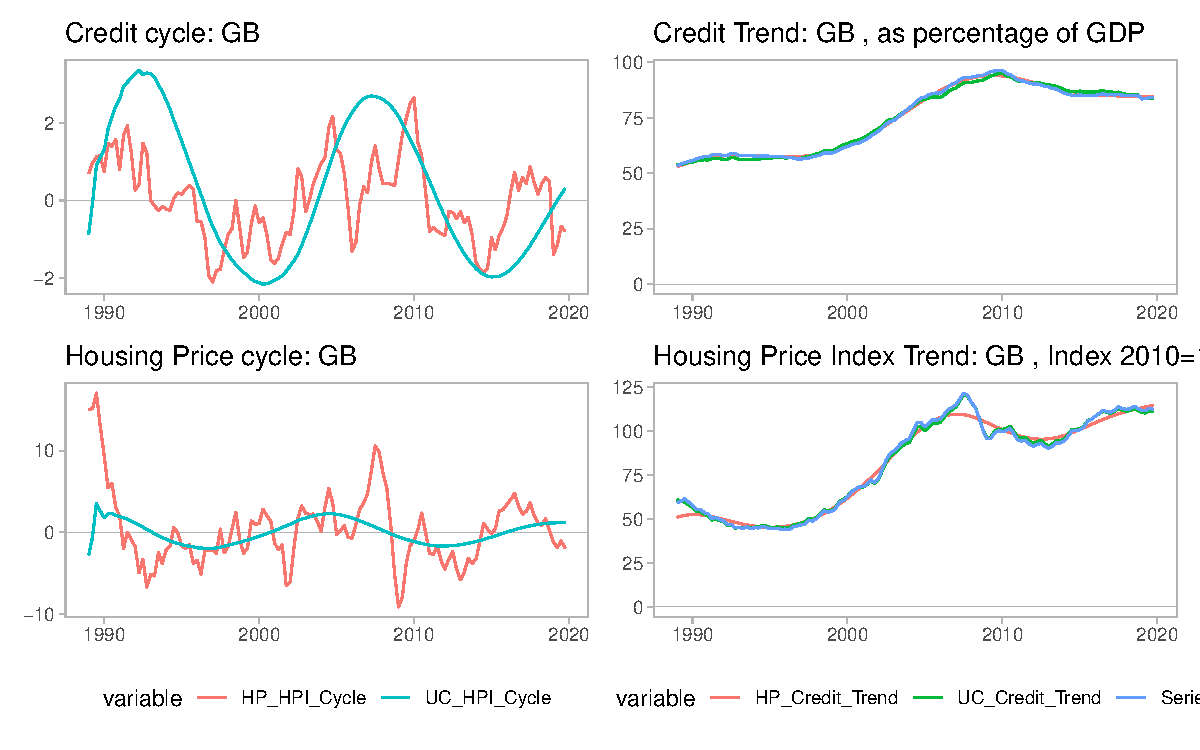
\includegraphics[scale=0.7]{../Graphs/Credit_cycle_GB.pdf}}
			\centerline{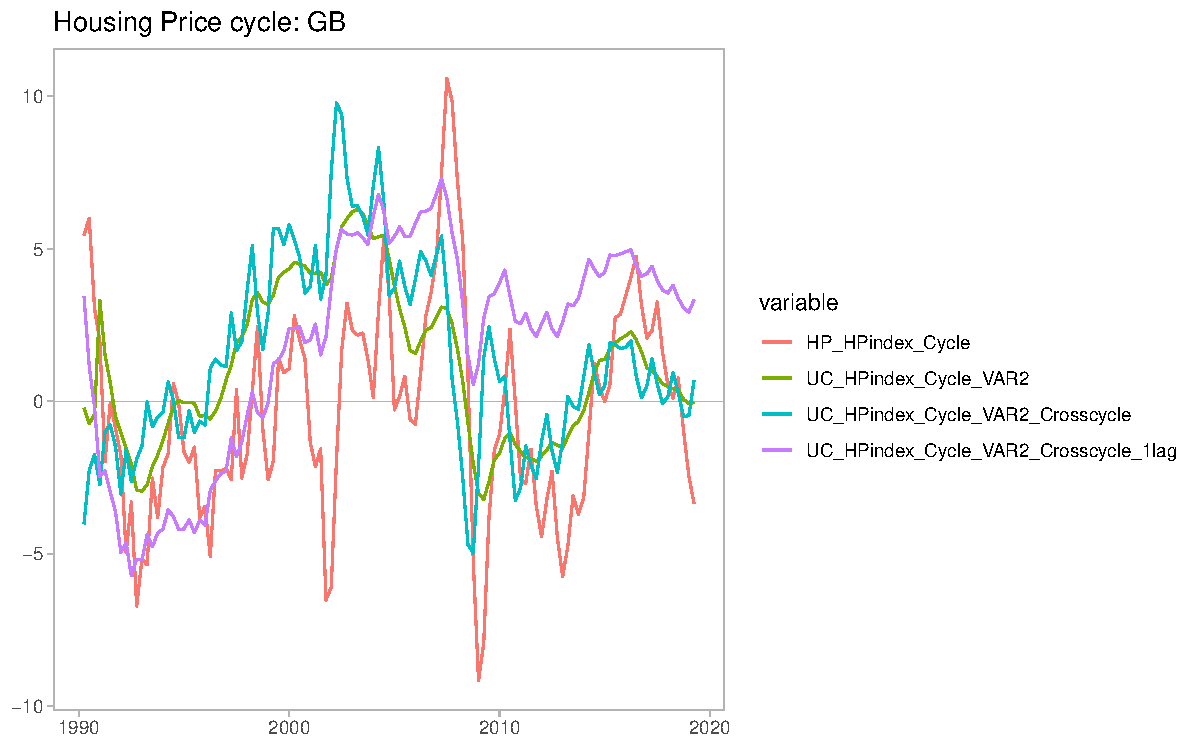
\includegraphics[scale=0.7]{../Graphs/HP_cycle_GB.pdf}}
		\end{figure}
		
		
		%
		%\begin{figure}[h!]
		%	\caption{Germany Credit components}	
		%	\centerline{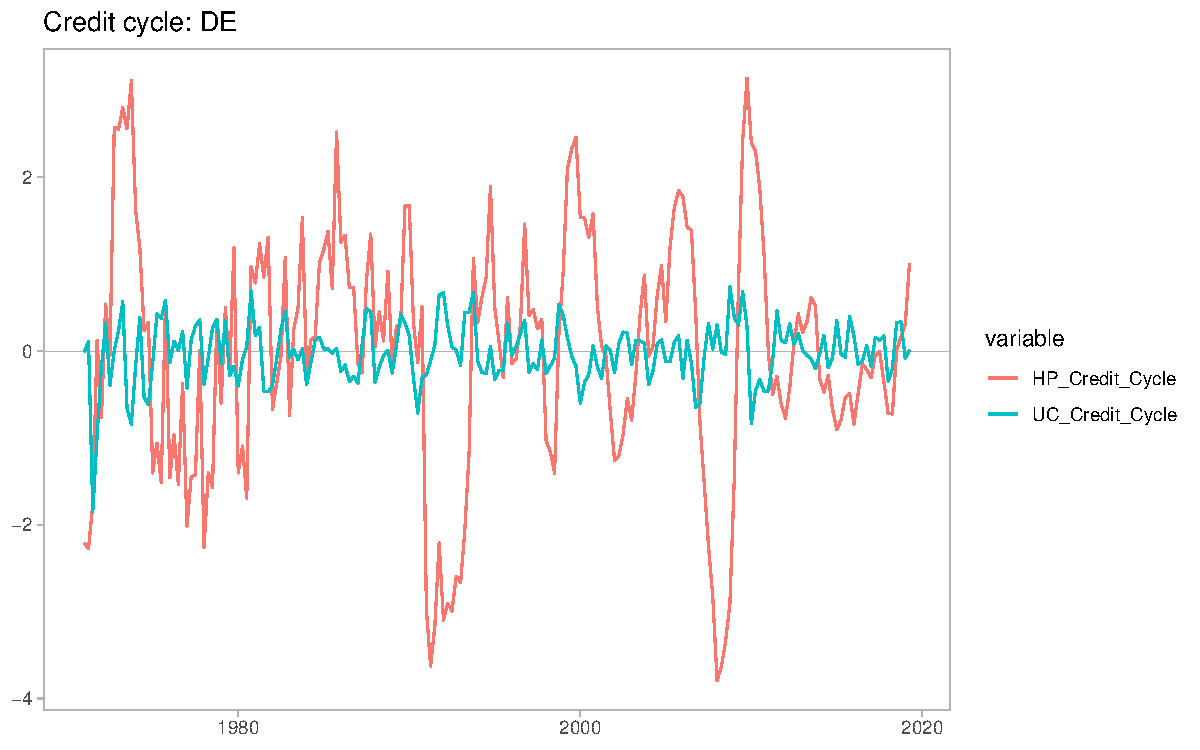
\includegraphics[scale=0.7]{../Output/Graphs/Credit_cycle_DE.pdf}}
		%	\centerline{\includegraphics[scale=0.7]{../Output/Graphs/Credit_trend_DE.pdf}}
		%\end{figure}
		%
		%\begin{figure}[h!]
		%	\caption{Germany Housing Price components}	
		%	\centerline{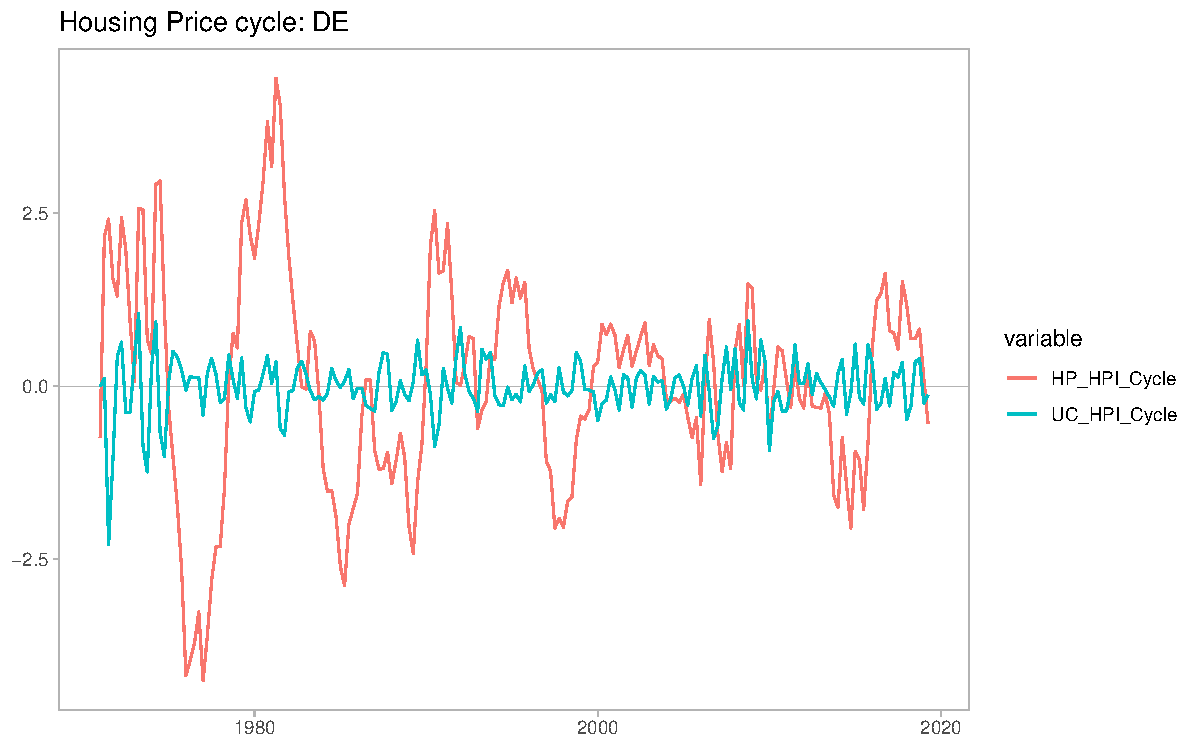
\includegraphics[scale=0.7]{../Output/Graphs/HP_cycle_DE.pdf}}
		%	\centerline{\includegraphics[scale=0.7]{../Output/Graphs/HP_trend_DE.pdf}}
		%\end{figure}
		%
		%
		%\begin{figure}[h!]
		%	\caption{France Credit components}	
		%	\centerline{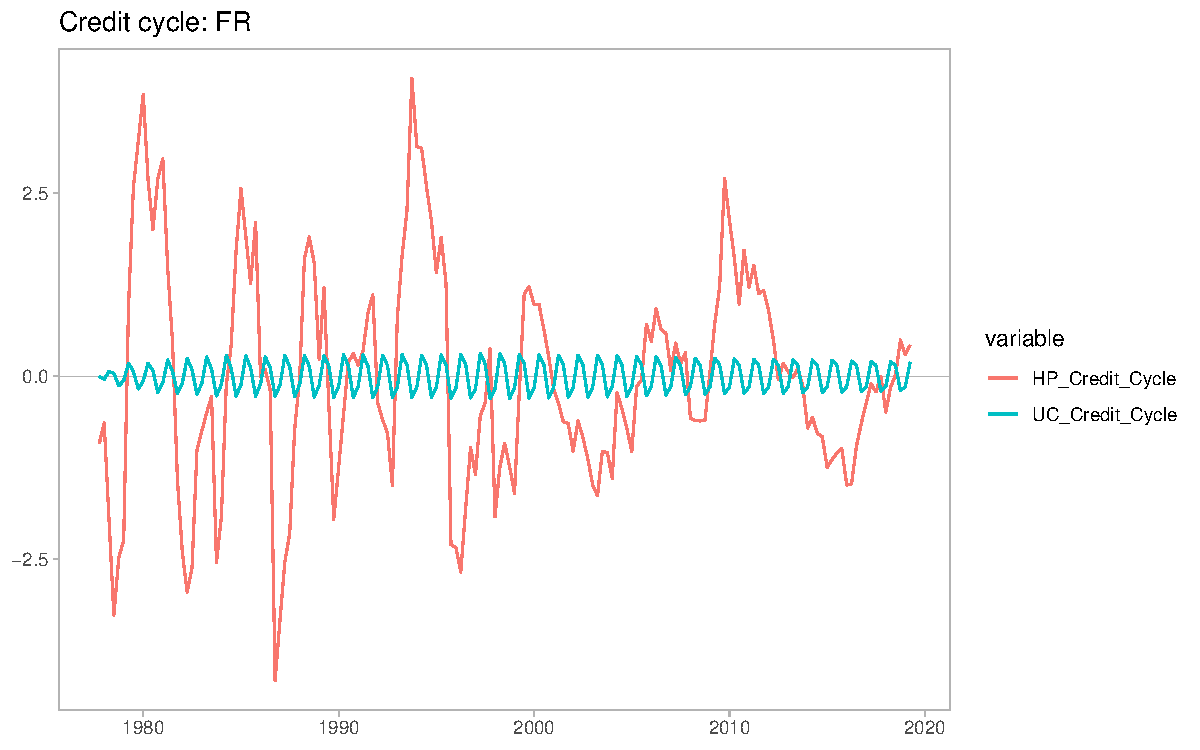
\includegraphics[scale=0.7]{../Output/Graphs/Credit_cycle_FR.pdf}}
		%	\centerline{\includegraphics[scale=0.7]{../Output/Graphs/Credit_trend_FR.pdf}}
		%\end{figure}
		%
		%\begin{figure}[h!]
		%	\caption{France Housing Price components}	
		%	\centerline{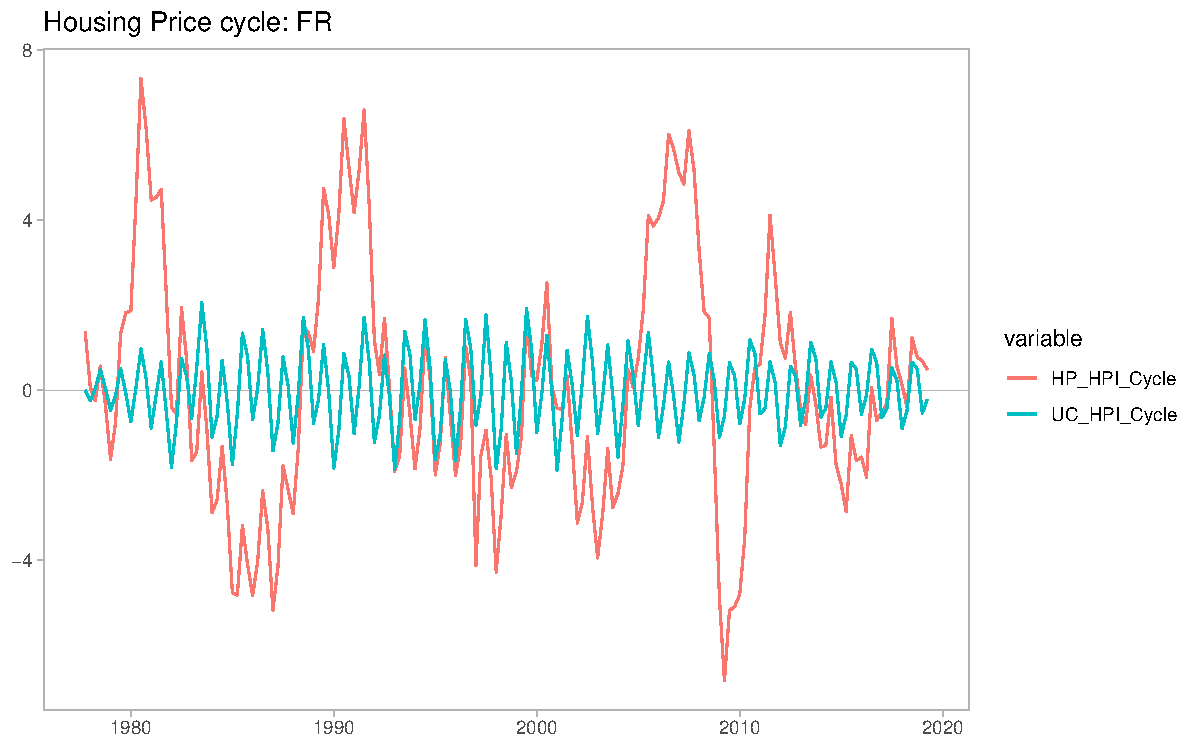
\includegraphics[scale=0.7]{../Output/Graphs/HP_cycle_FR.pdf}}
		%	\centerline{\includegraphics[scale=0.7]{../Output/Graphs/HP_trend_FR.pdf}}
		%\end{figure}
		%
		%
		%\begin{figure}[h!]
		%	\caption{Japan Credit components}	
		%	\centerline{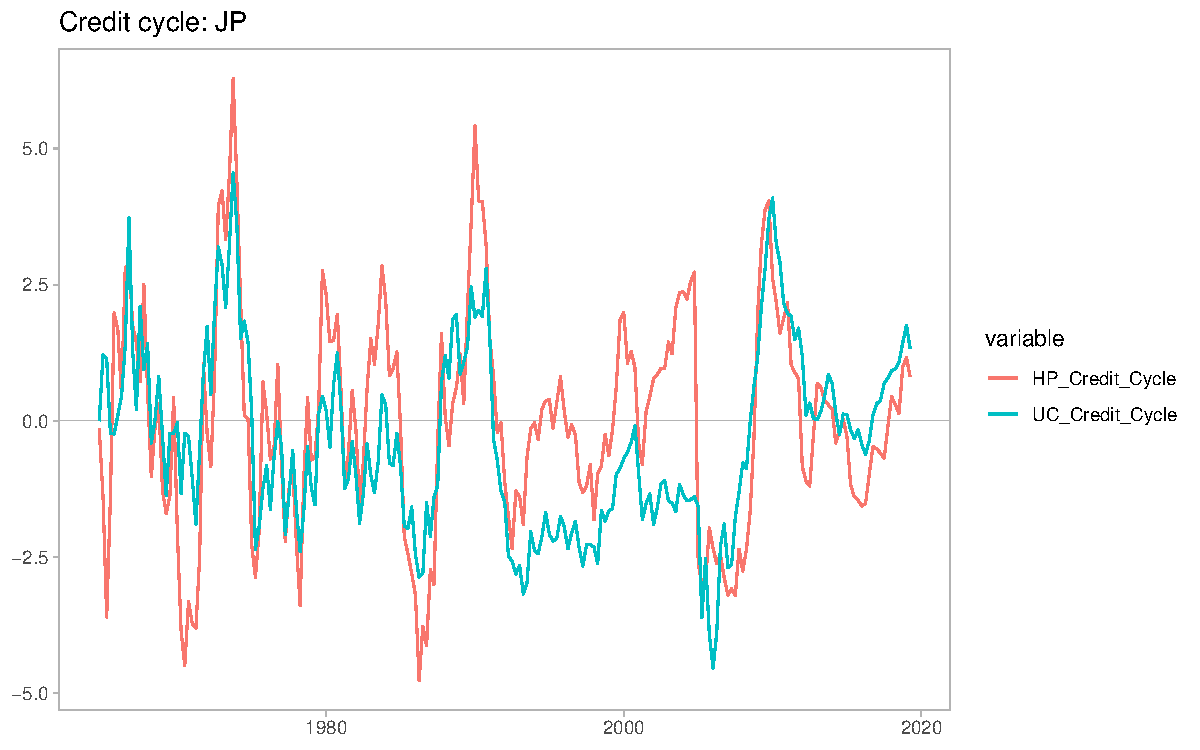
\includegraphics[scale=0.7]{../Output/Graphs/Credit_cycle_JP.pdf}}
		%	\centerline{\includegraphics[scale=0.7]{../Output/Graphs/Credit_trend_JP.pdf}}
		%\end{figure}
		%
		%\begin{figure}[h!]
		%	\caption{Japan Housing Price components}	
		%	\centerline{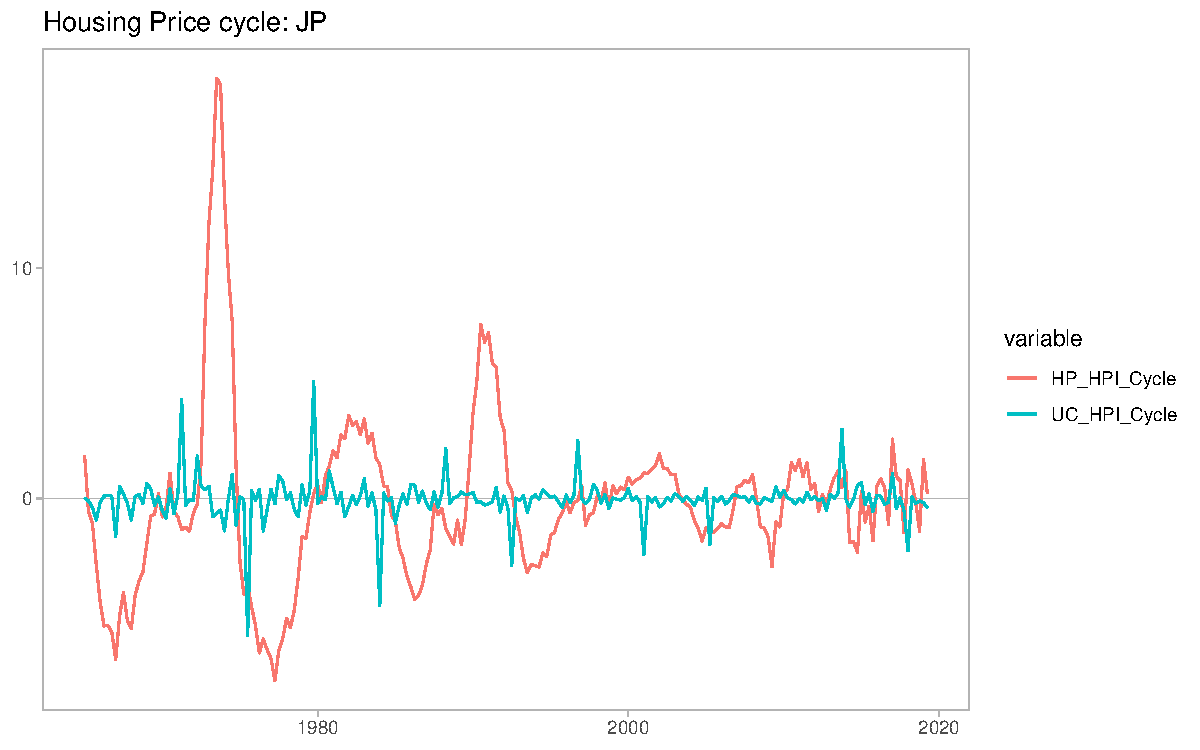
\includegraphics[scale=0.7]{../Output/Graphs/HP_cycle_JP.pdf}}
		%	\centerline{\includegraphics[scale=0.7]{../Output/Graphs/HP_trend_JP.pdf}}
		%\end{figure}
		%
		%
		%\begin{figure}[h!]
		%	\caption{Korea Credit components}	
		%	\centerline{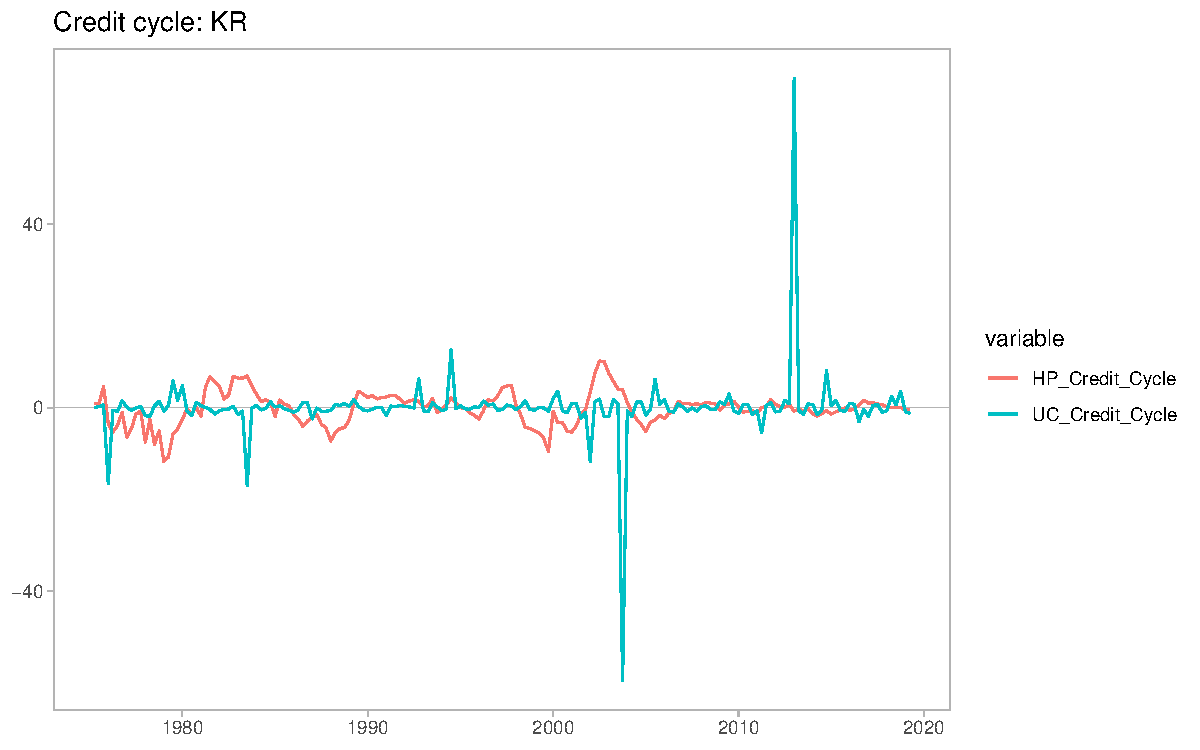
\includegraphics[scale=0.7]{../Output/Graphs/Credit_cycle_KR.pdf}}
		%	\centerline{\includegraphics[scale=0.7]{../Output/Graphs/Credit_trend_KR.pdf}}
		%\end{figure}
		%
		%\begin{figure}[h!]
		%	\caption{Korea Housing Price components}	
		%	\centerline{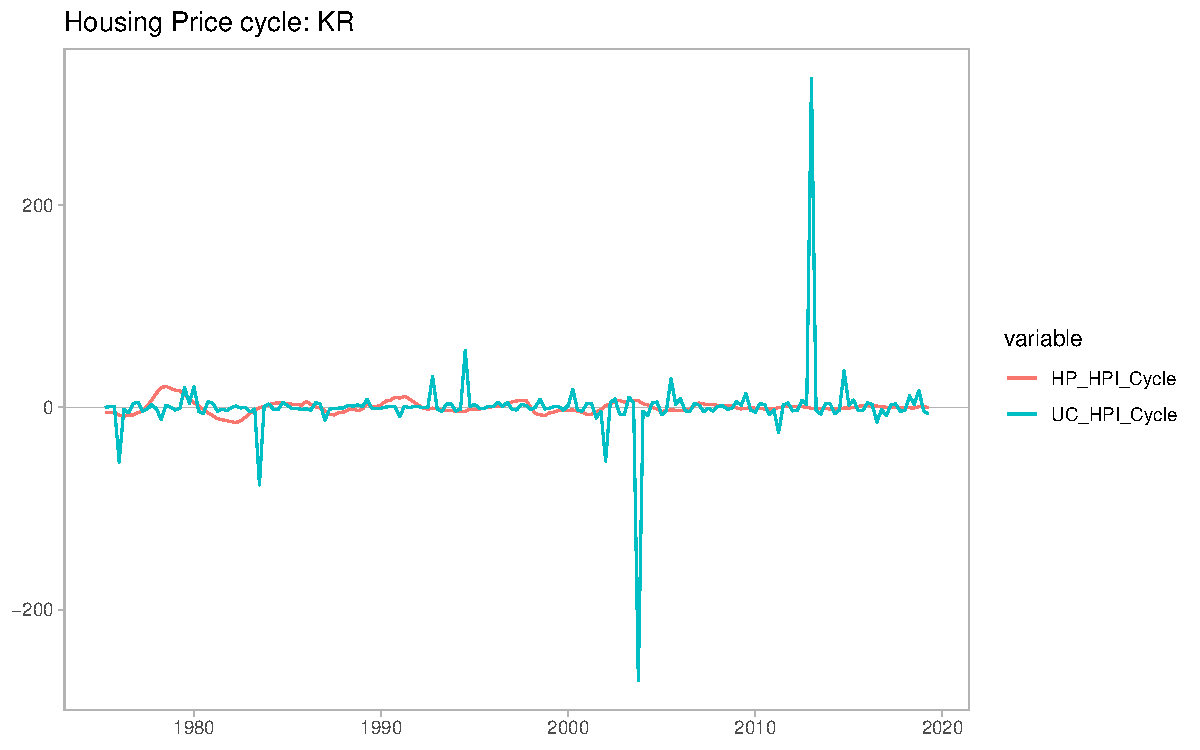
\includegraphics[scale=0.7]{../Output/Graphs/HP_cycle_KR.pdf}}
		%	\centerline{\includegraphics[scale=0.7]{../Output/Graphs/HP_trend_KR.pdf}}
		%\end{figure}
		
		\clearpage
		%
		%\section{Impulse Response Function}
		%
		%
		%
		%This section show IRFs that are really unstable. I am guessing that is because the way I specify the function:
		%
		%Instead of normally having: $\psi_t = \phi^y_{11}*\psi_l + \phi^y_{12}*\psi_{ll}$
		%
		%I specify the IRF as: $\psi_t = \phi^y_{11}*\psi_l + \phi^y_{12}*\psi_{ll} + \phi^y_{21}*\psi_l + \phi^y_{22}*\psi_{ll} $
		%\\
		%This potentially causes the unstability in the following IRF graphs. Also the fact that the constraints for autoregressive parameters have not been optimally setup could cause the issue.
		%
		%
		%\begin{figure}[h!]
		%	\caption{US IRF}	
		%	\centerline{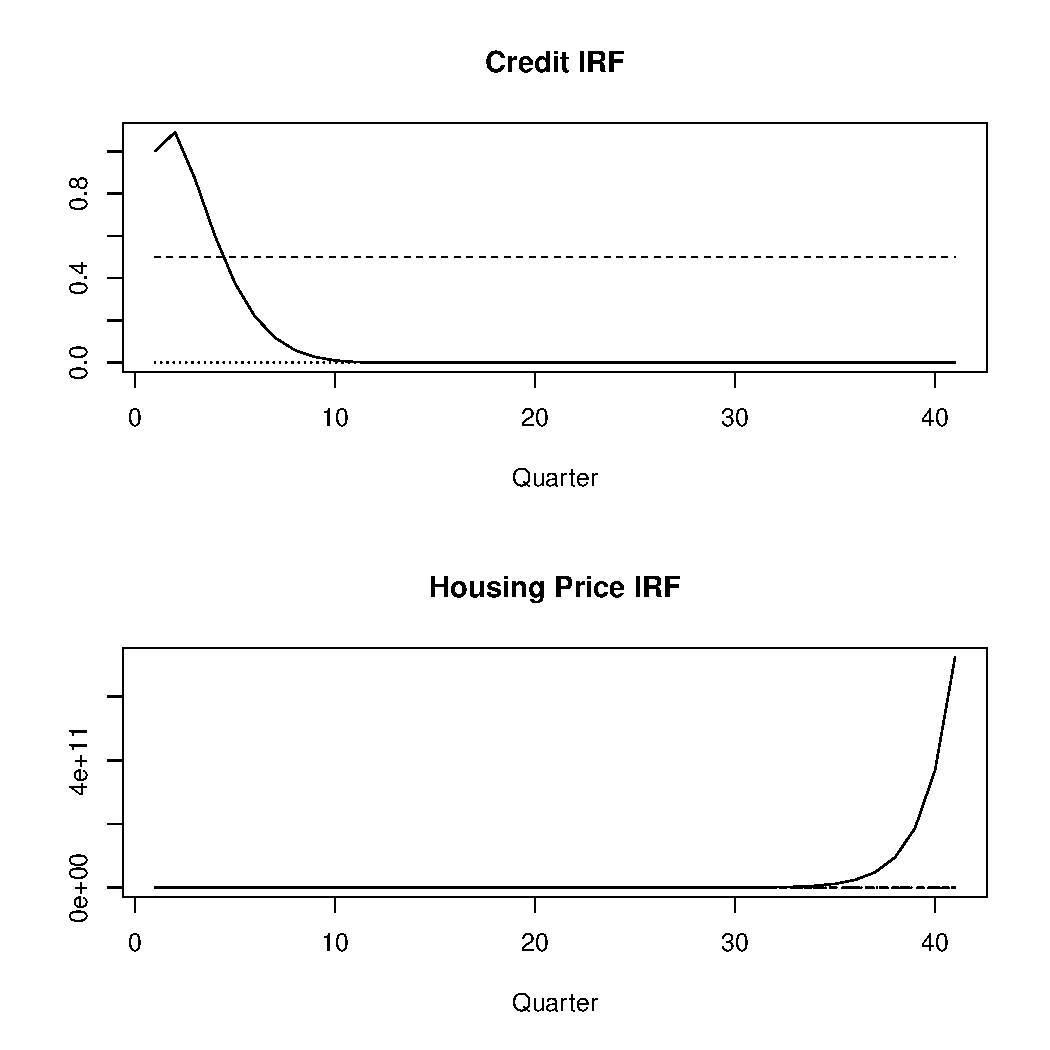
\includegraphics[scale=0.7]{../Output/Graphs/IRF_US.pdf}}
		%\end{figure}
		%
		%\begin{figure}[h!]
		%	\caption{UK IRF}	
		%	\centerline{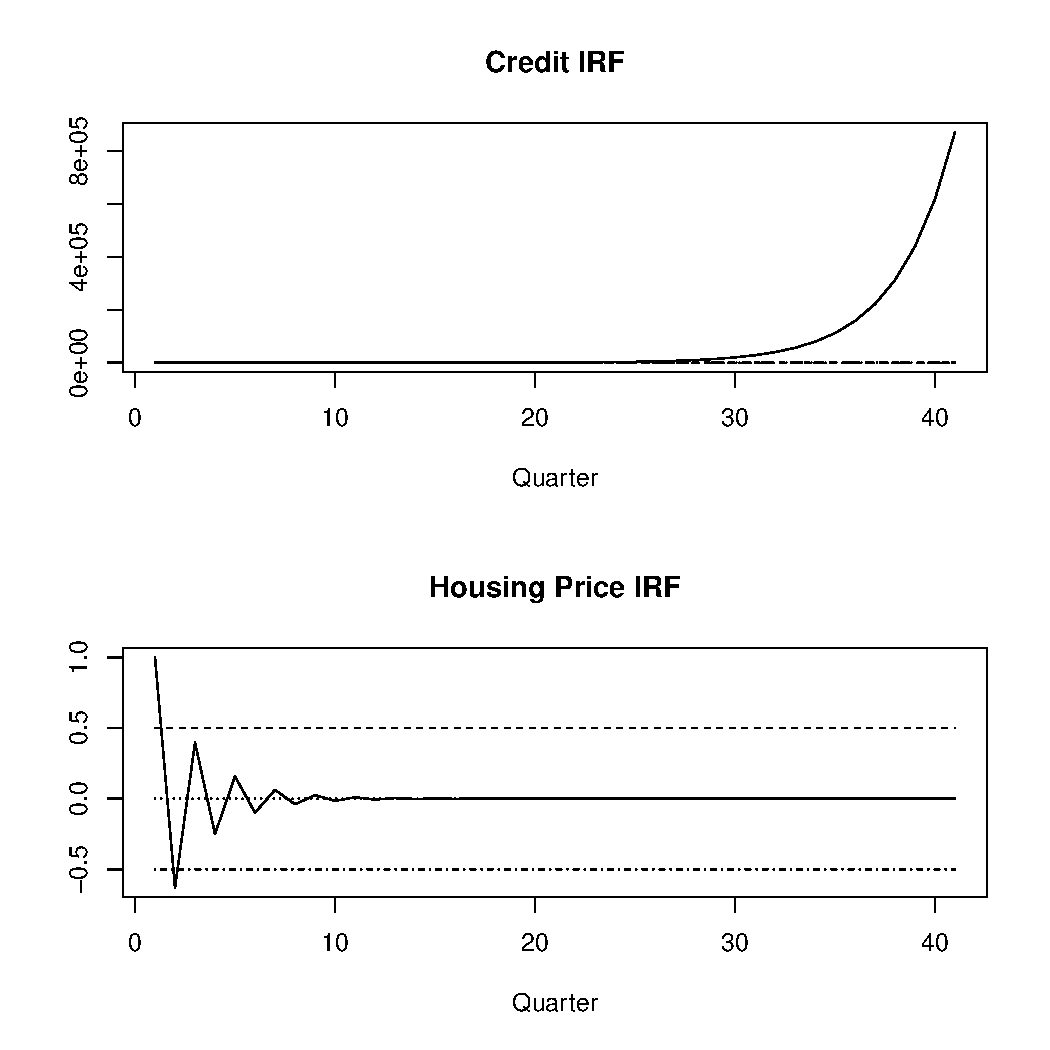
\includegraphics[scale=0.7]{../Output/Graphs/IRF_GB.pdf}}
		%\end{figure}
		%
		%\begin{figure}[h!]
		%	\caption{Germany IRF}	
		%	\centerline{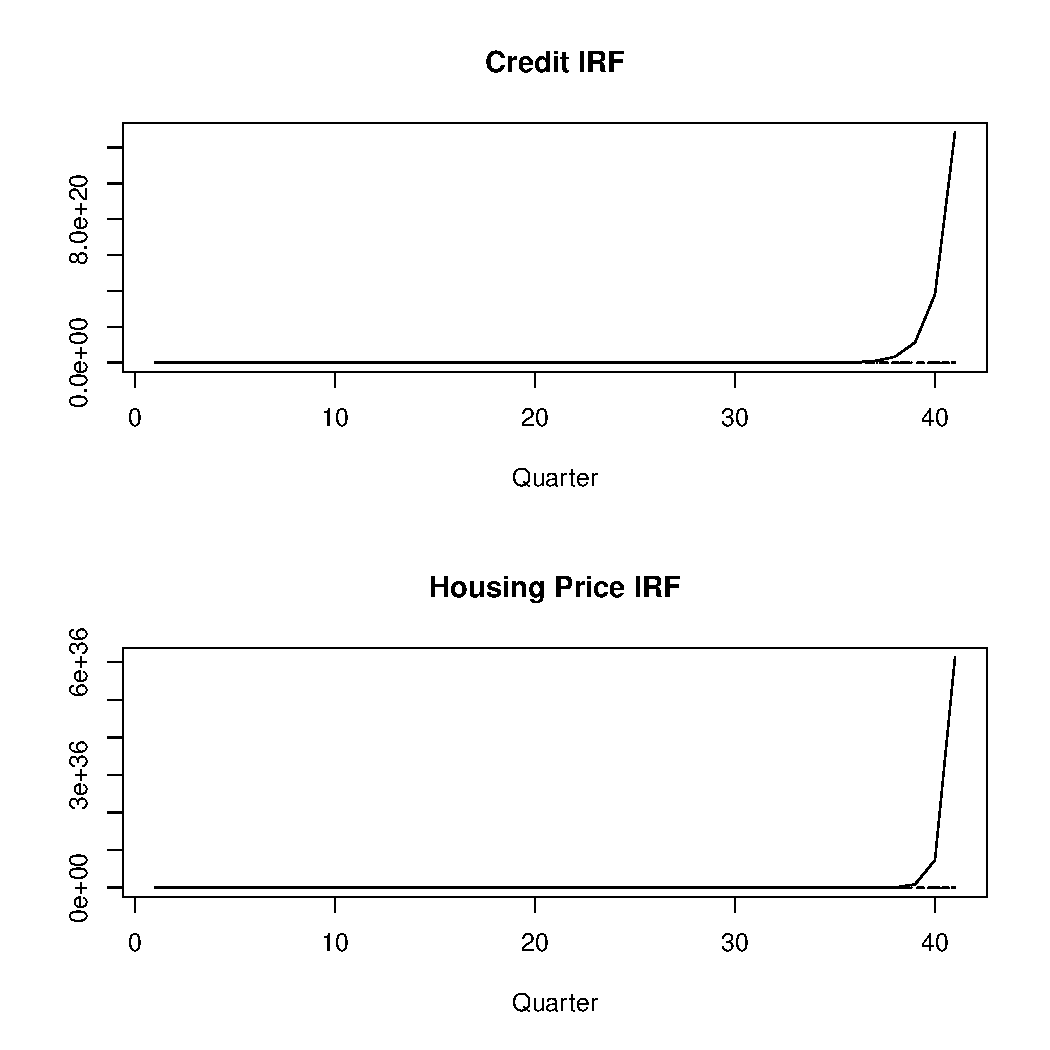
\includegraphics[scale=0.7]{../Output/Graphs/IRF_DE.pdf}}
		%\end{figure}
		%
		%\begin{figure}[h!]
		%	\caption{France IRF}	
		%	\centerline{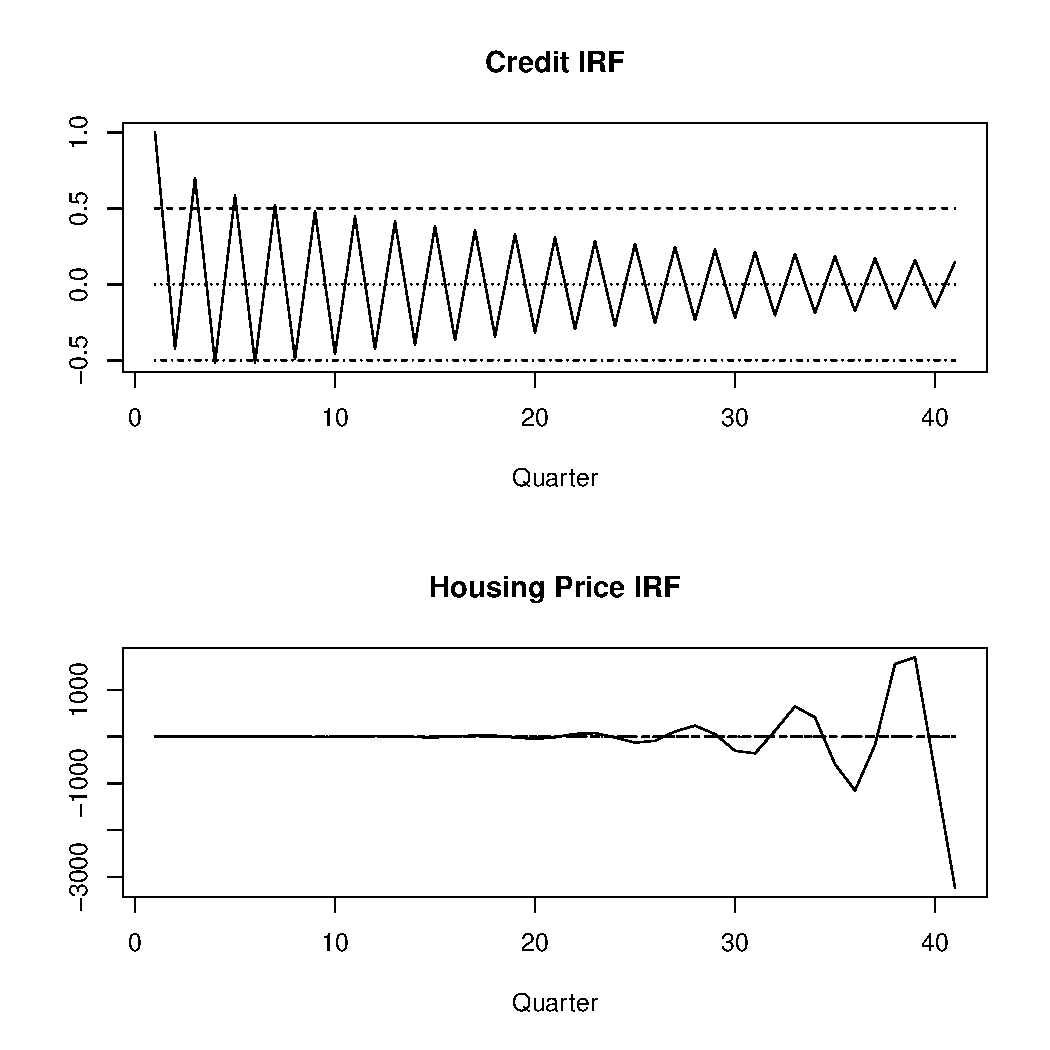
\includegraphics[scale=0.7]{../Output/Graphs/IRF_FR.pdf}}
		%\end{figure}
		%
		%\begin{figure}[h!]
		%	\caption{Japan IRF}	
		%	\centerline{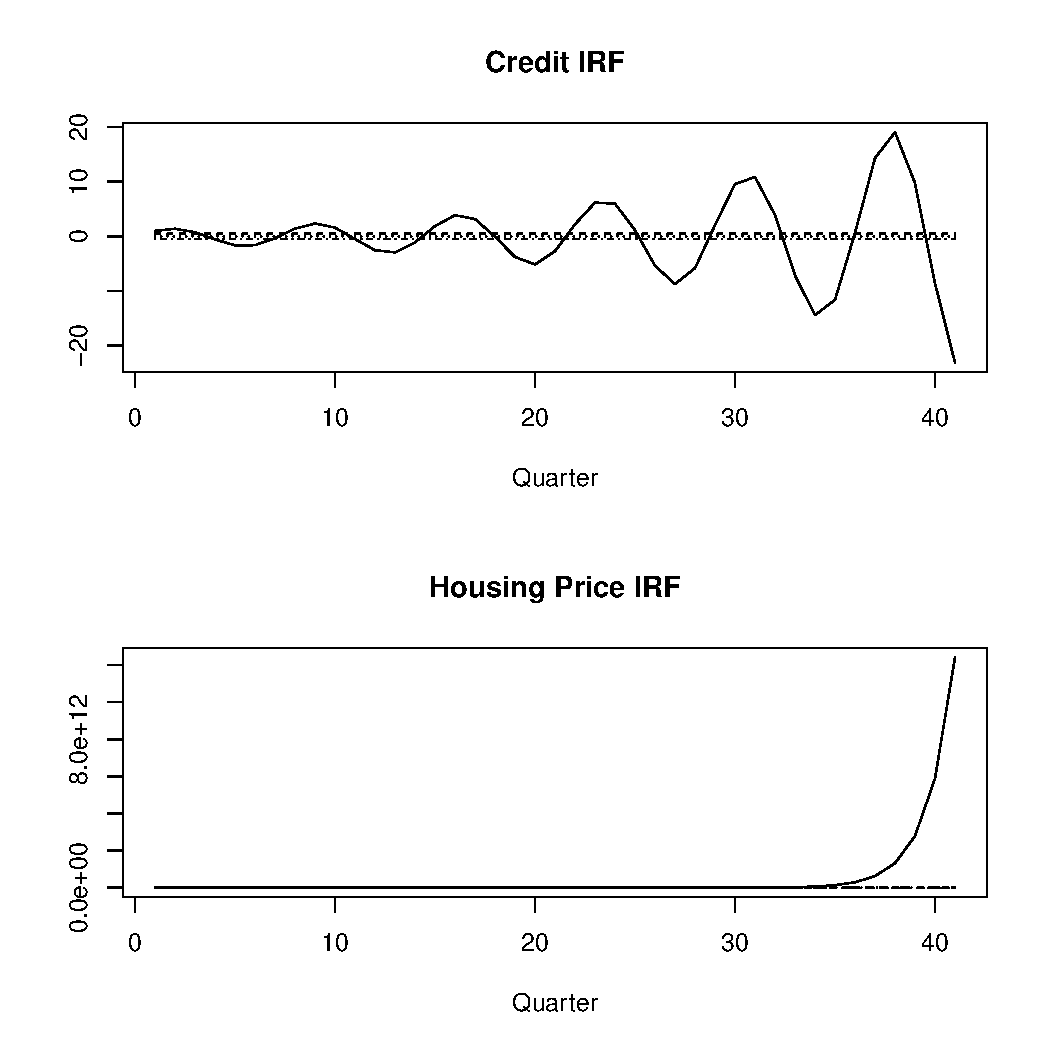
\includegraphics[scale=0.7]{../Output/Graphs/IRF_JP.pdf}}
		%\end{figure}
		%
		%\begin{figure}[h!]
		%	\caption{Korea IRF}	
		%	\centerline{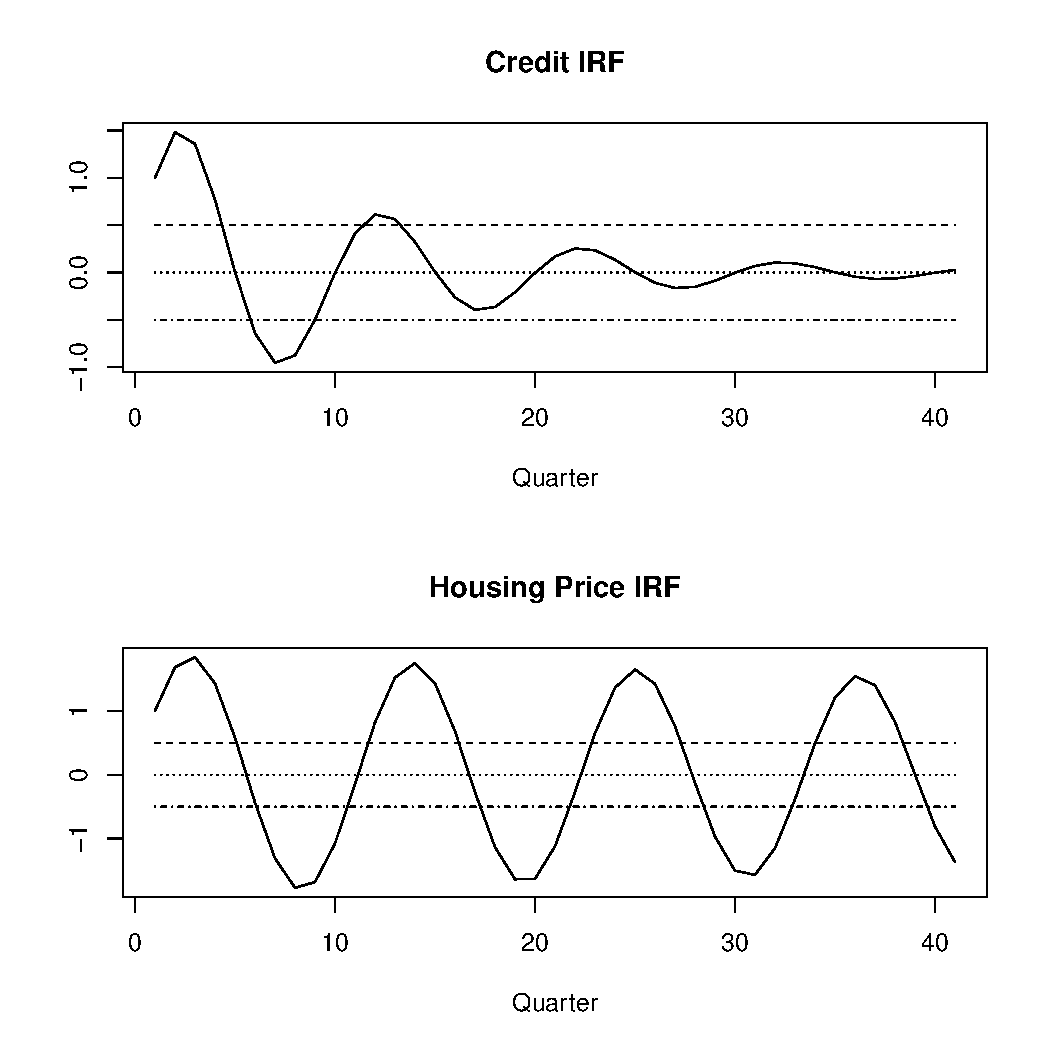
\includegraphics[scale=0.7]{../Output/Graphs/IRF_KR.pdf}}
		%\end{figure}
		
		
		
		
	\end{outline}
\end{document}